\documentclass[1p]{elsarticle_modified}
%\bibliographystyle{elsarticle-num}

%\usepackage[colorlinks]{hyperref}
%\usepackage{abbrmath_seonhwa} %\Abb, \Ascr, \Acal ,\Abf, \Afrak
\usepackage{amsfonts}
\usepackage{amssymb}
\usepackage{amsmath}
\usepackage{amsthm}
\usepackage{scalefnt}
\usepackage{amsbsy}
\usepackage{kotex}
\usepackage{caption}
\usepackage{subfig}
\usepackage{color}
\usepackage{graphicx}
\usepackage{xcolor} %% white, black, red, green, blue, cyan, magenta, yellow
\usepackage{float}
\usepackage{setspace}
\usepackage{hyperref}

\usepackage{tikz}
\usetikzlibrary{arrows}

\usepackage{multirow}
\usepackage{array} % fixed length table
\usepackage{hhline}

%%%%%%%%%%%%%%%%%%%%%
\makeatletter
\renewcommand*\env@matrix[1][\arraystretch]{%
	\edef\arraystretch{#1}%
	\hskip -\arraycolsep
	\let\@ifnextchar\new@ifnextchar
	\array{*\c@MaxMatrixCols c}}
\makeatother %https://tex.stackexchange.com/questions/14071/how-can-i-increase-the-line-spacing-in-a-matrix
%%%%%%%%%%%%%%%

\usepackage[normalem]{ulem}

\newcommand{\msout}[1]{\ifmmode\text{\sout{\ensuremath{#1}}}\else\sout{#1}\fi}
%SOURCE: \msout is \stkout macro in https://tex.stackexchange.com/questions/20609/strikeout-in-math-mode

\newcommand{\cancel}[1]{
	\ifmmode
	{\color{red}\msout{#1}}
	\else
	{\color{red}\sout{#1}}
	\fi
}

\newcommand{\add}[1]{
	{\color{blue}\uwave{#1}}
}

\newcommand{\replace}[2]{
	\ifmmode
	{\color{red}\msout{#1}}{\color{blue}\uwave{#2}}
	\else
	{\color{red}\sout{#1}}{\color{blue}\uwave{#2}}
	\fi
}

\newcommand{\Sol}{\mathcal{S}} %segment
\newcommand{\D}{D} %diagram
\newcommand{\A}{\mathcal{A}} %arc


%%%%%%%%%%%%%%%%%%%%%%%%%%%%%5 test

\def\sl{\operatorname{\textup{SL}}(2,\Cbb)}
\def\psl{\operatorname{\textup{PSL}}(2,\Cbb)}
\def\quan{\mkern 1mu \triangleright \mkern 1mu}

\theoremstyle{definition}
\newtheorem{thm}{Theorem}[section]
\newtheorem{prop}[thm]{Proposition}
\newtheorem{lem}[thm]{Lemma}
\newtheorem{ques}[thm]{Question}
\newtheorem{cor}[thm]{Corollary}
\newtheorem{defn}[thm]{Definition}
\newtheorem{exam}[thm]{Example}
\newtheorem{rmk}[thm]{Remark}
\newtheorem{alg}[thm]{Algorithm}

\newcommand{\I}{\sqrt{-1}}
\begin{document}

%\begin{frontmatter}
%
%\title{Boundary parabolic representations of knots up to 8 crossings}
%
%%% Group authors per affiliation:
%\author{Yunhi Cho} 
%\address{Department of Mathematics, University of Seoul, Seoul, Korea}
%\ead{yhcho@uos.ac.kr}
%
%
%\author{Seonhwa Kim} %\fnref{s_kim}}
%\address{Center for Geometry and Physics, Institute for Basic Science, Pohang, 37673, Korea}
%\ead{ryeona17@ibs.re.kr}
%
%\author{Hyuk Kim}
%\address{Department of Mathematical Sciences, Seoul National University, Seoul 08826, Korea}
%\ead{hyukkim@snu.ac.kr}
%
%\author{Seokbeom Yoon}
%\address{Department of Mathematical Sciences, Seoul National University, Seoul, 08826,  Korea}
%\ead{sbyoon15@snu.ac.kr}
%
%\begin{abstract}
%We find all boundary parabolic representation of knots up to 8 crossings.
%
%\end{abstract}
%\begin{keyword}
%    \MSC[2010] 57M25 
%\end{keyword}
%
%\end{frontmatter}

%\linenumbers
%\tableofcontents
%
\newcommand\colored[1]{\textcolor{white}{\rule[-0.35ex]{0.8em}{1.4ex}}\kern-0.8em\color{red} #1}%
%\newcommand\colored[1]{\textcolor{white}{ #1}\kern-2.17ex	\textcolor{white}{ #1}\kern-1.81ex	\textcolor{white}{ #1}\kern-2.15ex\color{red}#1	}

{\Large $\underline{12a_{1103}~(K12a_{1103})}$}

\setlength{\tabcolsep}{10pt}
\renewcommand{\arraystretch}{1.6}
\vspace{1cm}\begin{tabular}{m{100pt}>{\centering\arraybackslash}m{274pt}}
\multirow{5}{120pt}{
	\centering
	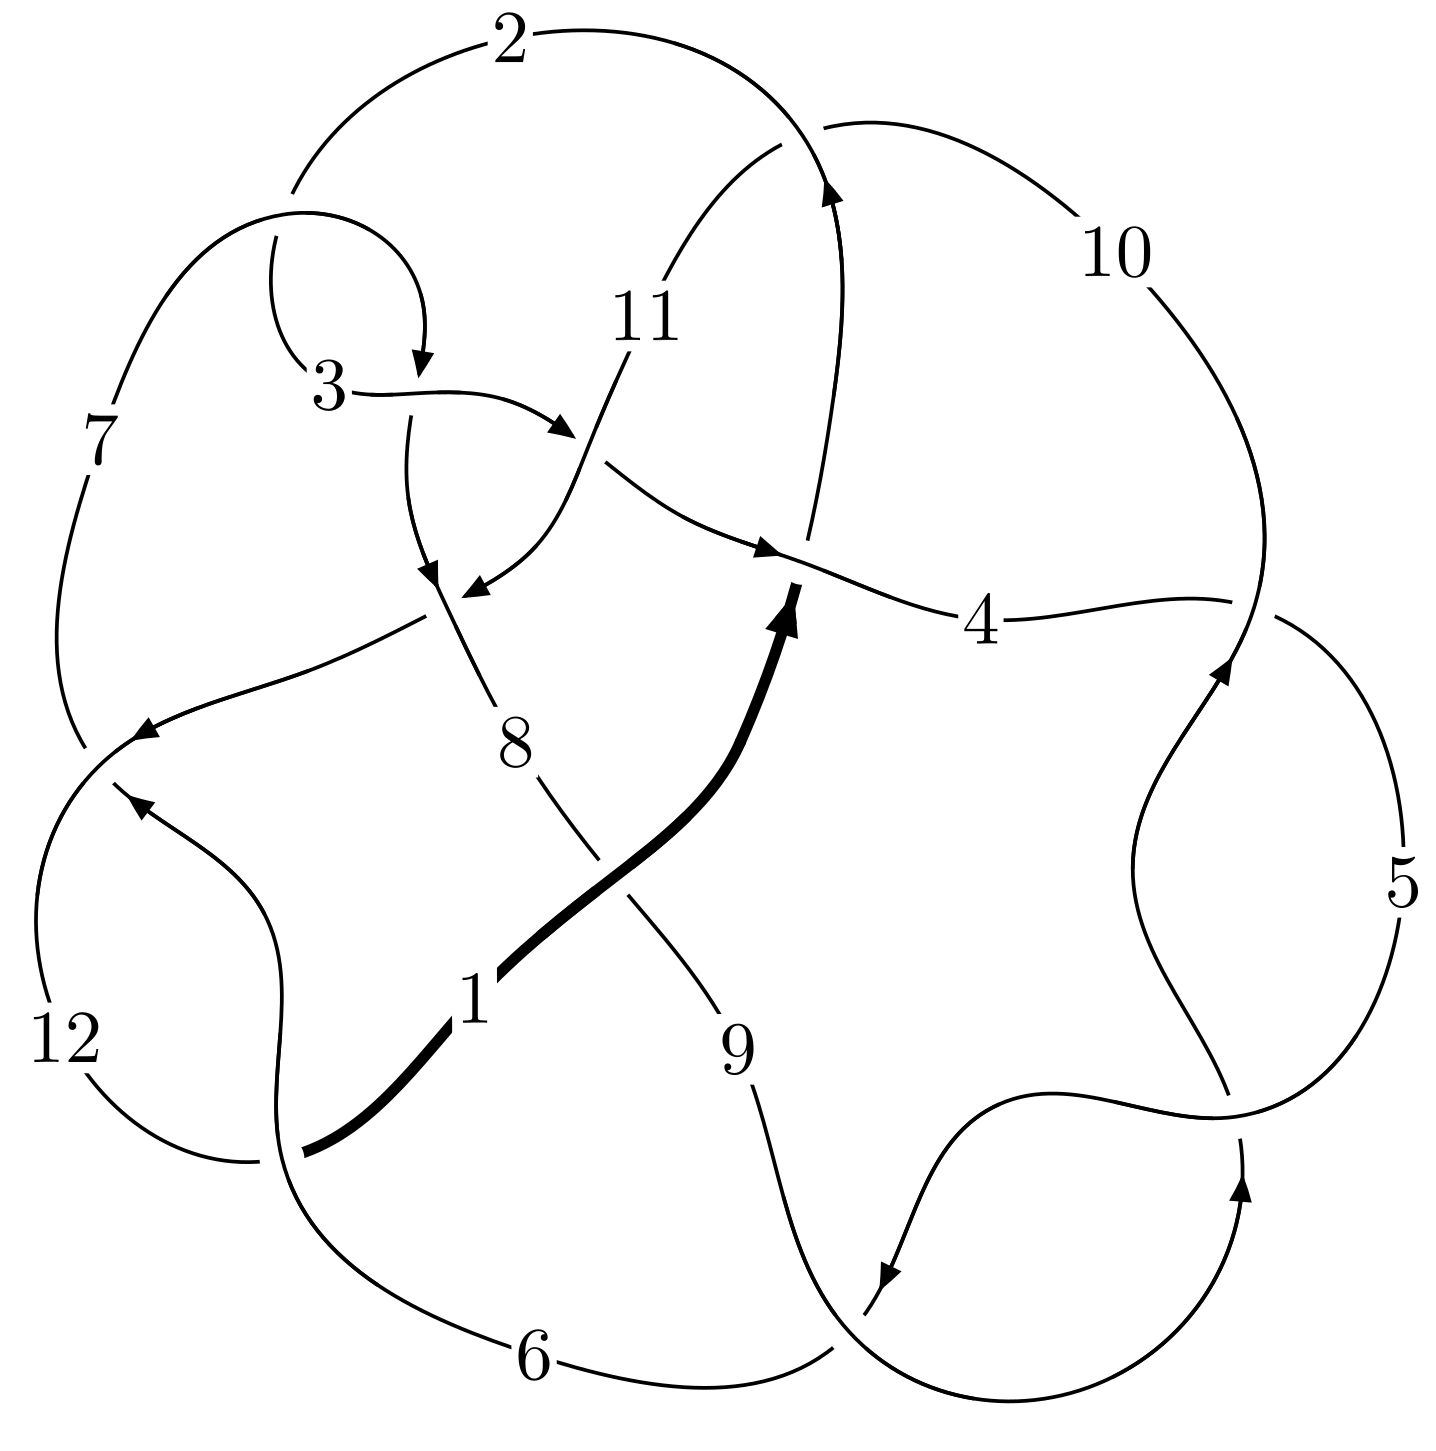
\includegraphics[width=112pt]{../../../GIT/diagram.site/Diagrams/png/1904_12a_1103.png}\\
\ \ \ A knot diagram\footnotemark}&
\allowdisplaybreaks
\textbf{Linearized knot diagam} \\
\cline{2-2}
 &
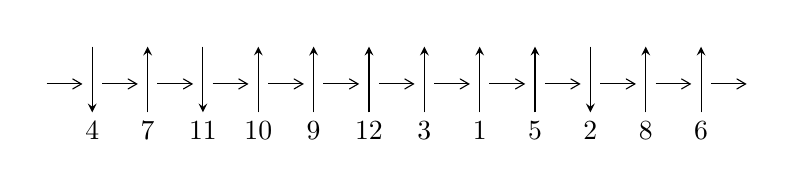
\begin{tikzpicture}[x=20pt, y=17pt]
	% nodes
	\node (C0) at (0, 0) {};
	\node (C1) at (1, 0) {};
	\node (C1U) at (1, +1) {};
	\node (C1D) at (1, -1) {4};

	\node (C2) at (2, 0) {};
	\node (C2U) at (2, +1) {};
	\node (C2D) at (2, -1) {7};

	\node (C3) at (3, 0) {};
	\node (C3U) at (3, +1) {};
	\node (C3D) at (3, -1) {11};

	\node (C4) at (4, 0) {};
	\node (C4U) at (4, +1) {};
	\node (C4D) at (4, -1) {10};

	\node (C5) at (5, 0) {};
	\node (C5U) at (5, +1) {};
	\node (C5D) at (5, -1) {9};

	\node (C6) at (6, 0) {};
	\node (C6U) at (6, +1) {};
	\node (C6D) at (6, -1) {12};

	\node (C7) at (7, 0) {};
	\node (C7U) at (7, +1) {};
	\node (C7D) at (7, -1) {3};

	\node (C8) at (8, 0) {};
	\node (C8U) at (8, +1) {};
	\node (C8D) at (8, -1) {1};

	\node (C9) at (9, 0) {};
	\node (C9U) at (9, +1) {};
	\node (C9D) at (9, -1) {5};

	\node (C10) at (10, 0) {};
	\node (C10U) at (10, +1) {};
	\node (C10D) at (10, -1) {2};

	\node (C11) at (11, 0) {};
	\node (C11U) at (11, +1) {};
	\node (C11D) at (11, -1) {8};

	\node (C12) at (12, 0) {};
	\node (C12U) at (12, +1) {};
	\node (C12D) at (12, -1) {6};
	\node (C13) at (13, 0) {};

	% arrows
	\draw[->,>={angle 60}]
	(C0) edge (C1) (C1) edge (C2) (C2) edge (C3) (C3) edge (C4) (C4) edge (C5) (C5) edge (C6) (C6) edge (C7) (C7) edge (C8) (C8) edge (C9) (C9) edge (C10) (C10) edge (C11) (C11) edge (C12) (C12) edge (C13) ;	\draw[->,>=stealth]
	(C1U) edge (C1D) (C2D) edge (C2U) (C3U) edge (C3D) (C4D) edge (C4U) (C5D) edge (C5U) (C6D) edge (C6U) (C7D) edge (C7U) (C8D) edge (C8U) (C9D) edge (C9U) (C10U) edge (C10D) (C11D) edge (C11U) (C12D) edge (C12U) ;
	\end{tikzpicture} \\
\hhline{~~} \\& 
\textbf{Solving Sequence} \\ \cline{2-2} 
 &
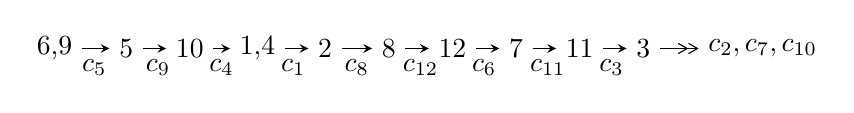
\begin{tikzpicture}[x=23pt, y=7pt]
	% node
	\node (A0) at (-1/8, 0) {6,9};
	\node (A1) at (1, 0) {5};
	\node (A2) at (2, 0) {10};
	\node (A3) at (49/16, 0) {1,4};
	\node (A4) at (33/8, 0) {2};
	\node (A5) at (41/8, 0) {8};
	\node (A6) at (49/8, 0) {12};
	\node (A7) at (57/8, 0) {7};
	\node (A8) at (65/8, 0) {11};
	\node (A9) at (73/8, 0) {3};
	\node (C1) at (1/2, -1) {$c_{5}$};
	\node (C2) at (3/2, -1) {$c_{9}$};
	\node (C3) at (5/2, -1) {$c_{4}$};
	\node (C4) at (29/8, -1) {$c_{1}$};
	\node (C5) at (37/8, -1) {$c_{8}$};
	\node (C6) at (45/8, -1) {$c_{12}$};
	\node (C7) at (53/8, -1) {$c_{6}$};
	\node (C8) at (61/8, -1) {$c_{11}$};
	\node (C9) at (69/8, -1) {$c_{3}$};
	\node (A10) at (11, 0) {$c_{2},c_{7},c_{10}$};

	% edge
	\draw[->,>=stealth]	
	(A0) edge (A1) (A1) edge (A2) (A2) edge (A3) (A3) edge (A4) (A4) edge (A5) (A5) edge (A6) (A6) edge (A7) (A7) edge (A8) (A8) edge (A9) ;
	\draw[->>,>={angle 60}]	
	(A9) edge (A10);
\end{tikzpicture} \\ 

\end{tabular} \\

\footnotetext{
The image of knot diagram is generated by the software ``\textbf{Draw programme}" developed by Andrew Bartholomew(\url{http://www.layer8.co.uk/maths/draw/index.htm\#Running-draw}), where we modified some parts for our purpose(\url{https://github.com/CATsTAILs/LinksPainter}).
}\phantom \\ \newline 
\centering \textbf{Ideals for irreducible components\footnotemark of $X_{\text{par}}$} 
 
\begin{align*}
I^u_{1}&=\langle 
6.61422\times10^{347} u^{121}-2.31862\times10^{348} u^{120}+\cdots+2.33758\times10^{350} b+1.43204\times10^{351},\\
\phantom{I^u_{1}}&\phantom{= \langle  }6.57060\times10^{349} u^{121}+1.89785\times10^{350} u^{120}+\cdots+3.66222\times10^{351} a-5.14072\times10^{352},\\
\phantom{I^u_{1}}&\phantom{= \langle  }u^{122}-2 u^{121}+\cdots-152 u-47\rangle \\
I^u_{2}&=\langle 
5203601 u^{24}-8655319 u^{23}+\cdots+2543847 b+13993811,\\
\phantom{I^u_{2}}&\phantom{= \langle  }1931569 u^{24}-2943707 u^{23}+\cdots+847949 a+3267199,\;u^{25}- u^{24}+\cdots+3 u+1\rangle \\
\\
\end{align*}
\raggedright * 2 irreducible components of $\dim_{\mathbb{C}}=0$, with total 147 representations.\\
\footnotetext{All coefficients of polynomials are rational numbers. But the coefficients are sometimes approximated in decimal forms when there is not enough margin.}
\newpage
\renewcommand{\arraystretch}{1}
\centering \section*{I. $I^u_{1}= \langle 6.61\times10^{347} u^{121}-2.32\times10^{348} u^{120}+\cdots+2.34\times10^{350} b+1.43\times10^{351},\;6.57\times10^{349} u^{121}+1.90\times10^{350} u^{120}+\cdots+3.66\times10^{351} a-5.14\times10^{352},\;u^{122}-2 u^{121}+\cdots-152 u-47 \rangle$}
\flushleft \textbf{(i) Arc colorings}\\
\begin{tabular}{m{7pt} m{180pt} m{7pt} m{180pt} }
\flushright $a_{6}=$&$\begin{pmatrix}1\\0\end{pmatrix}$ \\
\flushright $a_{9}=$&$\begin{pmatrix}0\\u\end{pmatrix}$ \\
\flushright $a_{5}=$&$\begin{pmatrix}1\\u^2\end{pmatrix}$ \\
\flushright $a_{10}=$&$\begin{pmatrix}u\\u^3+u\end{pmatrix}$ \\
\flushright $a_{1}=$&$\begin{pmatrix}-0.0179416 u^{121}-0.0518224 u^{120}+\cdots+69.8068 u+14.0372\\-0.00282951 u^{121}+0.00991885 u^{120}+\cdots-28.6098 u-6.12616\end{pmatrix}$ \\
\flushright $a_{4}=$&$\begin{pmatrix}u^2+1\\u^4+2 u^2\end{pmatrix}$ \\
\flushright $a_{2}=$&$\begin{pmatrix}0.00428493 u^{121}-0.0507703 u^{120}+\cdots+79.9417 u+15.7605\\-0.0155258 u^{121}+0.0135688 u^{120}+\cdots-27.5804 u-5.99751\end{pmatrix}$ \\
\flushright $a_{8}=$&$\begin{pmatrix}0.136734 u^{121}-0.432540 u^{120}+\cdots+9.98190 u+12.6345\\-0.0476945 u^{121}+0.180320 u^{120}+\cdots+1.25918 u-0.937436\end{pmatrix}$ \\
\flushright $a_{12}=$&$\begin{pmatrix}-0.0151121 u^{121}-0.0617412 u^{120}+\cdots+98.4166 u+20.1633\\-0.00282951 u^{121}+0.00991885 u^{120}+\cdots-28.6098 u-6.12616\end{pmatrix}$ \\
\flushright $a_{7}=$&$\begin{pmatrix}-0.0450192 u^{121}+0.0839493 u^{120}+\cdots+55.6338 u+2.64084\\0.0250738 u^{121}-0.0917528 u^{120}+\cdots-17.9308 u+1.65005\end{pmatrix}$ \\
\flushright $a_{11}=$&$\begin{pmatrix}0.00533299 u^{121}+0.0826627 u^{120}+\cdots+11.2409 u+8.99684\\-0.00257120 u^{121}-0.0401578 u^{120}+\cdots-5.20743 u-1.39274\end{pmatrix}$ \\
\flushright $a_{3}=$&$\begin{pmatrix}0.0525949 u^{121}-0.0614382 u^{120}+\cdots+95.0912 u+12.7763\\-0.0105100 u^{121}+0.0172075 u^{120}+\cdots-31.6028 u-1.95745\end{pmatrix}$\\&\end{tabular}
\flushleft \textbf{(ii) Obstruction class $= -1$}\\~\\
\flushleft \textbf{(iii) Cusp Shapes $= 0.328524 u^{121}-0.623159 u^{120}+\cdots-90.1165 u+22.2357$}\\~\\
\newpage\renewcommand{\arraystretch}{1}
\flushleft \textbf{(iv) u-Polynomials at the component}\newline \\
\begin{tabular}{m{50pt}|m{274pt}}
Crossings & \hspace{64pt}u-Polynomials at each crossing \\
\hline $$\begin{aligned}c_{1}\end{aligned}$$&$\begin{aligned}
&3(3 u^{122}-34 u^{121}+\cdots+928 u-64)
\end{aligned}$\\
\hline $$\begin{aligned}c_{2},c_{7}\end{aligned}$$&$\begin{aligned}
&u^{122}-31 u^{120}+\cdots+12944 u+3049
\end{aligned}$\\
\hline $$\begin{aligned}c_{3}\end{aligned}$$&$\begin{aligned}
&3(3 u^{122}- u^{121}+\cdots-5439 u-6578)
\end{aligned}$\\
\hline $$\begin{aligned}c_{4},c_{5},c_{9}\end{aligned}$$&$\begin{aligned}
&u^{122}-2 u^{121}+\cdots-152 u-47
\end{aligned}$\\
\hline $$\begin{aligned}c_{6},c_{12}\end{aligned}$$&$\begin{aligned}
&3(3 u^{122}+13 u^{121}+\cdots-10048 u-9856)
\end{aligned}$\\
\hline $$\begin{aligned}c_{8}\end{aligned}$$&$\begin{aligned}
&u^{122}+33 u^{120}+\cdots+43329371 u+6397761
\end{aligned}$\\
\hline $$\begin{aligned}c_{10}\end{aligned}$$&$\begin{aligned}
&u^{122}+4 u^{121}+\cdots+218080 u-15200
\end{aligned}$\\
\hline $$\begin{aligned}c_{11}\end{aligned}$$&$\begin{aligned}
&u^{122}+5 u^{121}+\cdots-286928 u+42477
\end{aligned}$\\
\hline
\end{tabular}\\~\\
\newpage\renewcommand{\arraystretch}{1}
\flushleft \textbf{(v) Riley Polynomials at the component}\newline \\
\begin{tabular}{m{50pt}|m{274pt}}
Crossings & \hspace{64pt}Riley Polynomials at each crossing \\
\hline $$\begin{aligned}c_{1}\end{aligned}$$&$\begin{aligned}
&9(9 y^{122}-178 y^{121}+\cdots-586752 y+4096)
\end{aligned}$\\
\hline $$\begin{aligned}c_{2},c_{7}\end{aligned}$$&$\begin{aligned}
&y^{122}-62 y^{121}+\cdots-249449374 y+9296401
\end{aligned}$\\
\hline $$\begin{aligned}c_{3}\end{aligned}$$&$\begin{aligned}
&9(9 y^{122}+323 y^{121}+\cdots+3.39707\times10^{9} y+4.32701\times10^{7})
\end{aligned}$\\
\hline $$\begin{aligned}c_{4},c_{5},c_{9}\end{aligned}$$&$\begin{aligned}
&y^{122}+134 y^{121}+\cdots+155026 y+2209
\end{aligned}$\\
\hline $$\begin{aligned}c_{6},c_{12}\end{aligned}$$&$\begin{aligned}
&9(9 y^{122}+887 y^{121}+\cdots+7.49242\times10^{9} y+9.71407\times10^{7})
\end{aligned}$\\
\hline $$\begin{aligned}c_{8}\end{aligned}$$&$\begin{aligned}
&y^{122}+66 y^{121}+\cdots+154006928978549 y+40931345813121
\end{aligned}$\\
\hline $$\begin{aligned}c_{10}\end{aligned}$$&$\begin{aligned}
&y^{122}-30 y^{121}+\cdots-15898137600 y+231040000
\end{aligned}$\\
\hline $$\begin{aligned}c_{11}\end{aligned}$$&$\begin{aligned}
&y^{122}-25 y^{121}+\cdots-64741944322 y+1804295529
\end{aligned}$\\
\hline
\end{tabular}\\~\\
\newpage\flushleft \textbf{(vi) Complex Volumes and Cusp Shapes}
$$\begin{array}{c|c|c}  
\text{Solutions to }I^u_{1}& \I (\text{vol} + \sqrt{-1}CS) & \text{Cusp shape}\\
 \hline 
\begin{aligned}
u &= -0.711563 + 0.720964 I \\
a &= -1.393790 + 0.166814 I \\
b &= -0.385156 + 1.286830 I\end{aligned}
 & -3.41596 - 8.34949 I & \phantom{-0.000000 } 0 \\ \hline\begin{aligned}
u &= -0.711563 - 0.720964 I \\
a &= -1.393790 - 0.166814 I \\
b &= -0.385156 - 1.286830 I\end{aligned}
 & -3.41596 + 8.34949 I & \phantom{-0.000000 } 0 \\ \hline\begin{aligned}
u &= -0.944407 + 0.213488 I \\
a &= \phantom{-}0.123892 + 0.730233 I \\
b &= \phantom{-}0.211045 + 1.169170 I\end{aligned}
 & -1.93761 + 3.07571 I & \phantom{-0.000000 } 0 \\ \hline\begin{aligned}
u &= -0.944407 - 0.213488 I \\
a &= \phantom{-}0.123892 - 0.730233 I \\
b &= \phantom{-}0.211045 - 1.169170 I\end{aligned}
 & -1.93761 - 3.07571 I & \phantom{-0.000000 } 0 \\ \hline\begin{aligned}
u &= -0.919192 + 0.571564 I \\
a &= \phantom{-}0.803946 - 0.667457 I \\
b &= \phantom{-}0.021906 - 1.351500 I\end{aligned}
 & -3.59564 - 3.96001 I & \phantom{-0.000000 } 0 \\ \hline\begin{aligned}
u &= -0.919192 - 0.571564 I \\
a &= \phantom{-}0.803946 + 0.667457 I \\
b &= \phantom{-}0.021906 + 1.351500 I\end{aligned}
 & -3.59564 + 3.96001 I & \phantom{-0.000000 } 0 \\ \hline\begin{aligned}
u &= \phantom{-}0.824964 + 0.703277 I \\
a &= \phantom{-}1.253070 + 0.282967 I \\
b &= \phantom{-}0.48146 + 1.38037 I\end{aligned}
 & -0.5307 + 14.4114 I & \phantom{-0.000000 } 0 \\ \hline\begin{aligned}
u &= \phantom{-}0.824964 - 0.703277 I \\
a &= \phantom{-}1.253070 - 0.282967 I \\
b &= \phantom{-}0.48146 - 1.38037 I\end{aligned}
 & -0.5307 - 14.4114 I & \phantom{-0.000000 } 0 \\ \hline\begin{aligned}
u &= \phantom{-}0.388492 + 1.015430 I \\
a &= -0.562166 - 0.618126 I \\
b &= \phantom{-}0.175635 - 1.239650 I\end{aligned}
 & -1.32108 - 2.03766 I & \phantom{-0.000000 } 0 \\ \hline\begin{aligned}
u &= \phantom{-}0.388492 - 1.015430 I \\
a &= -0.562166 + 0.618126 I \\
b &= \phantom{-}0.175635 + 1.239650 I\end{aligned}
 & -1.32108 + 2.03766 I & \phantom{-0.000000 } 0\\
 \hline 
 \end{array}$$\newpage$$\begin{array}{c|c|c}  
\text{Solutions to }I^u_{1}& \I (\text{vol} + \sqrt{-1}CS) & \text{Cusp shape}\\
 \hline 
\begin{aligned}
u &= -0.646003 + 0.637157 I \\
a &= -0.486912 - 0.920991 I \\
b &= -0.743569 + 0.184739 I\end{aligned}
 & \phantom{-}3.65027 + 4.40861 I & \phantom{-0.000000 } 0 \\ \hline\begin{aligned}
u &= -0.646003 - 0.637157 I \\
a &= -0.486912 + 0.920991 I \\
b &= -0.743569 - 0.184739 I\end{aligned}
 & \phantom{-}3.65027 - 4.40861 I & \phantom{-0.000000 } 0 \\ \hline\begin{aligned}
u &= -0.800406 + 0.779400 I \\
a &= \phantom{-}0.869349 - 0.273565 I \\
b &= \phantom{-}0.242672 - 1.354910 I\end{aligned}
 & -4.15358 - 2.18179 I & \phantom{-0.000000 } 0 \\ \hline\begin{aligned}
u &= -0.800406 - 0.779400 I \\
a &= \phantom{-}0.869349 + 0.273565 I \\
b &= \phantom{-}0.242672 + 1.354910 I\end{aligned}
 & -4.15358 + 2.18179 I & \phantom{-0.000000 } 0 \\ \hline\begin{aligned}
u &= \phantom{-}0.875561 + 0.742822 I \\
a &= -0.828938 - 0.268010 I \\
b &= -0.434435 - 1.182230 I\end{aligned}
 & -3.28469 + 5.56042 I & \phantom{-0.000000 } 0 \\ \hline\begin{aligned}
u &= \phantom{-}0.875561 - 0.742822 I \\
a &= -0.828938 + 0.268010 I \\
b &= -0.434435 + 1.182230 I\end{aligned}
 & -3.28469 - 5.56042 I & \phantom{-0.000000 } 0 \\ \hline\begin{aligned}
u &= \phantom{-}1.075060 + 0.432573 I \\
a &= \phantom{-}0.034159 + 0.686221 I \\
b &= -0.340366 + 1.218210 I\end{aligned}
 & \phantom{-}0.40180 - 8.35687 I & \phantom{-0.000000 } 0 \\ \hline\begin{aligned}
u &= \phantom{-}1.075060 - 0.432573 I \\
a &= \phantom{-}0.034159 - 0.686221 I \\
b &= -0.340366 - 1.218210 I\end{aligned}
 & \phantom{-}0.40180 + 8.35687 I & \phantom{-0.000000 } 0 \\ \hline\begin{aligned}
u &= -0.144300 + 0.809129 I \\
a &= -0.07390 - 1.72418 I \\
b &= -0.285127 + 0.727893 I\end{aligned}
 & \phantom{-}3.40823 - 2.43241 I & \phantom{-0.000000 } 0 \\ \hline\begin{aligned}
u &= -0.144300 - 0.809129 I \\
a &= -0.07390 + 1.72418 I \\
b &= -0.285127 - 0.727893 I\end{aligned}
 & \phantom{-}3.40823 + 2.43241 I & \phantom{-0.000000 } 0\\
 \hline 
 \end{array}$$\newpage$$\begin{array}{c|c|c}  
\text{Solutions to }I^u_{1}& \I (\text{vol} + \sqrt{-1}CS) & \text{Cusp shape}\\
 \hline 
\begin{aligned}
u &= \phantom{-}0.966543 + 0.696539 I \\
a &= -0.601302 - 0.495746 I \\
b &= \phantom{-}0.088758 - 1.105320 I\end{aligned}
 & -2.99662 + 0.99837 I & \phantom{-0.000000 } 0 \\ \hline\begin{aligned}
u &= \phantom{-}0.966543 - 0.696539 I \\
a &= -0.601302 + 0.495746 I \\
b &= \phantom{-}0.088758 + 1.105320 I\end{aligned}
 & -2.99662 - 0.99837 I & \phantom{-0.000000 } 0 \\ \hline\begin{aligned}
u &= -0.671198 + 0.449572 I \\
a &= \phantom{-}1.228040 + 0.056946 I \\
b &= \phantom{-}1.102320 - 0.119184 I\end{aligned}
 & \phantom{-}4.15580 - 8.88626 I & \phantom{-0.000000 } 0 \\ \hline\begin{aligned}
u &= -0.671198 - 0.449572 I \\
a &= \phantom{-}1.228040 - 0.056946 I \\
b &= \phantom{-}1.102320 + 0.119184 I\end{aligned}
 & \phantom{-}4.15580 + 8.88626 I & \phantom{-0.000000 } 0 \\ \hline\begin{aligned}
u &= \phantom{-}0.592638 + 0.541840 I \\
a &= \phantom{-}0.098411 + 0.973133 I \\
b &= -0.285793 + 0.805911 I\end{aligned}
 & \phantom{-}2.81379 - 0.15458 I & \phantom{-0.000000 } 0 \\ \hline\begin{aligned}
u &= \phantom{-}0.592638 - 0.541840 I \\
a &= \phantom{-}0.098411 - 0.973133 I \\
b &= -0.285793 - 0.805911 I\end{aligned}
 & \phantom{-}2.81379 + 0.15458 I & \phantom{-0.000000 } 0 \\ \hline\begin{aligned}
u &= -0.110720 + 1.199860 I \\
a &= -0.140904 + 1.236810 I \\
b &= \phantom{-}0.238007 - 0.355608 I\end{aligned}
 & \phantom{-}1.82109 + 0.39807 I & \phantom{-0.000000 } 0 \\ \hline\begin{aligned}
u &= -0.110720 - 1.199860 I \\
a &= -0.140904 - 1.236810 I \\
b &= \phantom{-}0.238007 + 0.355608 I\end{aligned}
 & \phantom{-}1.82109 - 0.39807 I & \phantom{-0.000000 } 0 \\ \hline\begin{aligned}
u &= \phantom{-}0.620141 + 0.482366 I \\
a &= \phantom{-}1.65587 + 0.57045 I \\
b &= \phantom{-}0.458721 + 0.949845 I\end{aligned}
 & \phantom{-}2.97710 + 4.30693 I & \phantom{-0.000000 } 0 \\ \hline\begin{aligned}
u &= \phantom{-}0.620141 - 0.482366 I \\
a &= \phantom{-}1.65587 - 0.57045 I \\
b &= \phantom{-}0.458721 - 0.949845 I\end{aligned}
 & \phantom{-}2.97710 - 4.30693 I & \phantom{-0.000000 } 0\\
 \hline 
 \end{array}$$\newpage$$\begin{array}{c|c|c}  
\text{Solutions to }I^u_{1}& \I (\text{vol} + \sqrt{-1}CS) & \text{Cusp shape}\\
 \hline 
\begin{aligned}
u &= \phantom{-}0.552575 + 0.547041 I \\
a &= -1.134450 + 0.309121 I \\
b &= -0.782083 - 0.025889 I\end{aligned}
 & \phantom{-}0.65822 + 4.07057 I & \phantom{-0.000000 } 0 \\ \hline\begin{aligned}
u &= \phantom{-}0.552575 - 0.547041 I \\
a &= -1.134450 - 0.309121 I \\
b &= -0.782083 + 0.025889 I\end{aligned}
 & \phantom{-}0.65822 - 4.07057 I & \phantom{-0.000000 } 0 \\ \hline\begin{aligned}
u &= -0.504759 + 0.574242 I \\
a &= \phantom{-}0.573223 - 0.402914 I \\
b &= -0.025420 - 1.288960 I\end{aligned}
 & -2.90797 - 1.31424 I & \phantom{-0.000000 } 0 \\ \hline\begin{aligned}
u &= -0.504759 - 0.574242 I \\
a &= \phantom{-}0.573223 + 0.402914 I \\
b &= -0.025420 + 1.288960 I\end{aligned}
 & -2.90797 + 1.31424 I & \phantom{-0.000000 } 0 \\ \hline\begin{aligned}
u &= -0.166628 + 1.260070 I \\
a &= \phantom{-}0.499290 + 0.246247 I \\
b &= \phantom{-}0.48725 - 1.51603 I\end{aligned}
 & -3.71841 - 1.26400 I & \phantom{-0.000000 } 0 \\ \hline\begin{aligned}
u &= -0.166628 - 1.260070 I \\
a &= \phantom{-}0.499290 - 0.246247 I \\
b &= \phantom{-}0.48725 + 1.51603 I\end{aligned}
 & -3.71841 + 1.26400 I & \phantom{-0.000000 } 0 \\ \hline\begin{aligned}
u &= \phantom{-}0.593443 + 0.357252 I \\
a &= \phantom{-}0.978294 - 0.576018 I \\
b &= \phantom{-}0.560470 + 0.099085 I\end{aligned}
 & \phantom{-}1.193900 - 0.193638 I & \phantom{-0.000000 } 0 \\ \hline\begin{aligned}
u &= \phantom{-}0.593443 - 0.357252 I \\
a &= \phantom{-}0.978294 + 0.576018 I \\
b &= \phantom{-}0.560470 - 0.099085 I\end{aligned}
 & \phantom{-}1.193900 + 0.193638 I & \phantom{-0.000000 } 0 \\ \hline\begin{aligned}
u &= -0.168599 + 0.648321 I \\
a &= -0.295148 + 0.830971 I \\
b &= \phantom{-}0.191511 - 1.052380 I\end{aligned}
 & -2.45670 - 1.73198 I & \phantom{-0.000000 } 0 \\ \hline\begin{aligned}
u &= -0.168599 - 0.648321 I \\
a &= -0.295148 - 0.830971 I \\
b &= \phantom{-}0.191511 + 1.052380 I\end{aligned}
 & -2.45670 + 1.73198 I & \phantom{-0.000000 } 0\\
 \hline 
 \end{array}$$\newpage$$\begin{array}{c|c|c}  
\text{Solutions to }I^u_{1}& \I (\text{vol} + \sqrt{-1}CS) & \text{Cusp shape}\\
 \hline 
\begin{aligned}
u &= -0.363565 + 0.560558 I \\
a &= \phantom{-}1.77768 + 0.49343 I \\
b &= \phantom{-}0.106654 - 1.301380 I\end{aligned}
 & -3.17722 - 2.12113 I & \phantom{-0.000000 } 0 \\ \hline\begin{aligned}
u &= -0.363565 - 0.560558 I \\
a &= \phantom{-}1.77768 - 0.49343 I \\
b &= \phantom{-}0.106654 + 1.301380 I\end{aligned}
 & -3.17722 + 2.12113 I & \phantom{-0.000000 } 0 \\ \hline\begin{aligned}
u &= \phantom{-}0.644624 + 0.168603 I \\
a &= -1.50186 - 1.79693 I \\
b &= -0.318245 - 1.260090 I\end{aligned}
 & \phantom{-}1.20438 + 5.87556 I & \phantom{-0.000000 } 0 \\ \hline\begin{aligned}
u &= \phantom{-}0.644624 - 0.168603 I \\
a &= -1.50186 + 1.79693 I \\
b &= -0.318245 + 1.260090 I\end{aligned}
 & \phantom{-}1.20438 - 5.87556 I & \phantom{-0.000000 } 0 \\ \hline\begin{aligned}
u &= \phantom{-}0.529634 + 0.380291 I \\
a &= \phantom{-}0.76835 + 1.42293 I \\
b &= -0.286234 + 0.353485 I\end{aligned}
 & \phantom{-}1.79521 + 4.30982 I & \phantom{-}6.00000 - 6.96880 I \\ \hline\begin{aligned}
u &= \phantom{-}0.529634 - 0.380291 I \\
a &= \phantom{-}0.76835 - 1.42293 I \\
b &= -0.286234 - 0.353485 I\end{aligned}
 & \phantom{-}1.79521 - 4.30982 I & \phantom{-}6.00000 + 6.96880 I \\ \hline\begin{aligned}
u &= -0.068350 + 1.354020 I \\
a &= \phantom{-}0.879519 + 0.471079 I \\
b &= \phantom{-}0.894615 - 0.037123 I\end{aligned}
 & \phantom{-}0.37227 - 3.90700 I & \phantom{-0.000000 } 0 \\ \hline\begin{aligned}
u &= -0.068350 - 1.354020 I \\
a &= \phantom{-}0.879519 - 0.471079 I \\
b &= \phantom{-}0.894615 + 0.037123 I\end{aligned}
 & \phantom{-}0.37227 + 3.90700 I & \phantom{-0.000000 } 0 \\ \hline\begin{aligned}
u &= \phantom{-}0.221459 + 0.578403 I \\
a &= \phantom{-}1.83852 + 0.27944 I \\
b &= \phantom{-}0.55654 + 1.33372 I\end{aligned}
 & -1.51959 + 7.61336 I & \phantom{-}1.31895 - 8.06220 I \\ \hline\begin{aligned}
u &= \phantom{-}0.221459 - 0.578403 I \\
a &= \phantom{-}1.83852 - 0.27944 I \\
b &= \phantom{-}0.55654 - 1.33372 I\end{aligned}
 & -1.51959 - 7.61336 I & \phantom{-}1.31895 + 8.06220 I\\
 \hline 
 \end{array}$$\newpage$$\begin{array}{c|c|c}  
\text{Solutions to }I^u_{1}& \I (\text{vol} + \sqrt{-1}CS) & \text{Cusp shape}\\
 \hline 
\begin{aligned}
u &= \phantom{-}0.14969 + 1.41637 I \\
a &= \phantom{-}1.71834 - 0.45136 I \\
b &= \phantom{-}0.394011 + 1.307680 I\end{aligned}
 & -3.83496 + 8.49001 I & \phantom{-0.000000 } 0 \\ \hline\begin{aligned}
u &= \phantom{-}0.14969 - 1.41637 I \\
a &= \phantom{-}1.71834 + 0.45136 I \\
b &= \phantom{-}0.394011 - 1.307680 I\end{aligned}
 & -3.83496 - 8.49001 I & \phantom{-0.000000 } 0 \\ \hline\begin{aligned}
u &= \phantom{-}0.08472 + 1.44133 I \\
a &= -0.408149 + 0.109054 I \\
b &= -2.15366 - 0.96195 I\end{aligned}
 & -4.10524 + 0.35227 I & \phantom{-0.000000 } 0 \\ \hline\begin{aligned}
u &= \phantom{-}0.08472 - 1.44133 I \\
a &= -0.408149 - 0.109054 I \\
b &= -2.15366 + 0.96195 I\end{aligned}
 & -4.10524 - 0.35227 I & \phantom{-0.000000 } 0 \\ \hline\begin{aligned}
u &= \phantom{-}0.397137 + 0.364224 I \\
a &= \phantom{-}0.998842 + 0.493503 I \\
b &= \phantom{-}0.963377 + 0.544778 I\end{aligned}
 & \phantom{-}1.60418 - 1.28589 I & \phantom{-}5.39014 - 4.42202 I \\ \hline\begin{aligned}
u &= \phantom{-}0.397137 - 0.364224 I \\
a &= \phantom{-}0.998842 - 0.493503 I \\
b &= \phantom{-}0.963377 - 0.544778 I\end{aligned}
 & \phantom{-}1.60418 + 1.28589 I & \phantom{-}5.39014 + 4.42202 I \\ \hline\begin{aligned}
u &= -0.179399 + 0.501683 I \\
a &= -2.23272 + 0.79175 I \\
b &= -0.375239 + 1.137740 I\end{aligned}
 & -4.44948 - 1.35368 I & -3.38262 + 9.54178 I \\ \hline\begin{aligned}
u &= -0.179399 - 0.501683 I \\
a &= -2.23272 - 0.79175 I \\
b &= -0.375239 - 1.137740 I\end{aligned}
 & -4.44948 + 1.35368 I & -3.38262 - 9.54178 I \\ \hline\begin{aligned}
u &= \phantom{-}0.08929 + 1.47252 I \\
a &= -0.608189 + 0.288110 I \\
b &= -0.513432 - 0.573870 I\end{aligned}
 & -4.41097 + 1.90052 I & \phantom{-0.000000 } 0 \\ \hline\begin{aligned}
u &= \phantom{-}0.08929 - 1.47252 I \\
a &= -0.608189 - 0.288110 I \\
b &= -0.513432 + 0.573870 I\end{aligned}
 & -4.41097 - 1.90052 I & \phantom{-0.000000 } 0\\
 \hline 
 \end{array}$$\newpage$$\begin{array}{c|c|c}  
\text{Solutions to }I^u_{1}& \I (\text{vol} + \sqrt{-1}CS) & \text{Cusp shape}\\
 \hline 
\begin{aligned}
u &= -0.361732 + 0.376917 I \\
a &= -0.671912 + 0.745291 I \\
b &= -0.266762 - 0.217897 I\end{aligned}
 & -1.38502 - 1.11204 I & -1.01179 + 2.65936 I \\ \hline\begin{aligned}
u &= -0.361732 - 0.376917 I \\
a &= -0.671912 - 0.745291 I \\
b &= -0.266762 + 0.217897 I\end{aligned}
 & -1.38502 + 1.11204 I & -1.01179 - 2.65936 I \\ \hline\begin{aligned}
u &= \phantom{-}0.01380 + 1.48140 I \\
a &= -0.071801 - 0.845889 I \\
b &= \phantom{-}0.05954 + 1.99044 I\end{aligned}
 & -6.47523 + 0.96880 I & \phantom{-0.000000 } 0 \\ \hline\begin{aligned}
u &= \phantom{-}0.01380 - 1.48140 I \\
a &= -0.071801 + 0.845889 I \\
b &= \phantom{-}0.05954 - 1.99044 I\end{aligned}
 & -6.47523 - 0.96880 I & \phantom{-0.000000 } 0 \\ \hline\begin{aligned}
u &= -0.08734 + 1.48047 I \\
a &= -0.645293 - 0.186675 I \\
b &= -1.180530 - 0.503207 I\end{aligned}
 & -1.50030 - 1.09339 I & \phantom{-0.000000 } 0 \\ \hline\begin{aligned}
u &= -0.08734 - 1.48047 I \\
a &= -0.645293 + 0.186675 I \\
b &= -1.180530 + 0.503207 I\end{aligned}
 & -1.50030 + 1.09339 I & \phantom{-0.000000 } 0 \\ \hline\begin{aligned}
u &= -0.375684 + 0.349981 I \\
a &= \phantom{-}1.77959 + 0.54451 I \\
b &= \phantom{-}0.834764 + 0.478037 I\end{aligned}
 & \phantom{-}4.56255 + 0.46430 I & \phantom{-}12.30374 + 4.04241 I \\ \hline\begin{aligned}
u &= -0.375684 - 0.349981 I \\
a &= \phantom{-}1.77959 - 0.54451 I \\
b &= \phantom{-}0.834764 - 0.478037 I\end{aligned}
 & \phantom{-}4.56255 - 0.46430 I & \phantom{-}12.30374 - 4.04241 I \\ \hline\begin{aligned}
u &= \phantom{-}0.17535 + 1.47846 I \\
a &= -1.091770 - 0.334682 I \\
b &= -0.156136 - 0.434741 I\end{aligned}
 & -4.29256 + 6.88236 I & \phantom{-0.000000 } 0 \\ \hline\begin{aligned}
u &= \phantom{-}0.17535 - 1.47846 I \\
a &= -1.091770 + 0.334682 I \\
b &= -0.156136 + 0.434741 I\end{aligned}
 & -4.29256 - 6.88236 I & \phantom{-0.000000 } 0\\
 \hline 
 \end{array}$$\newpage$$\begin{array}{c|c|c}  
\text{Solutions to }I^u_{1}& \I (\text{vol} + \sqrt{-1}CS) & \text{Cusp shape}\\
 \hline 
\begin{aligned}
u &= -0.00805 + 1.50090 I \\
a &= -1.35168 + 1.39321 I \\
b &= \phantom{-}0.013083 - 1.194870 I\end{aligned}
 & -6.76650 - 6.68366 I & \phantom{-0.000000 } 0 \\ \hline\begin{aligned}
u &= -0.00805 - 1.50090 I \\
a &= -1.35168 - 1.39321 I \\
b &= \phantom{-}0.013083 + 1.194870 I\end{aligned}
 & -6.76650 + 6.68366 I & \phantom{-0.000000 } 0 \\ \hline\begin{aligned}
u &= -0.11115 + 1.49746 I \\
a &= \phantom{-}0.721143 - 0.197957 I \\
b &= \phantom{-}0.731066 + 0.108932 I\end{aligned}
 & -7.65579 - 2.81845 I & \phantom{-0.000000 } 0 \\ \hline\begin{aligned}
u &= -0.11115 - 1.49746 I \\
a &= \phantom{-}0.721143 + 0.197957 I \\
b &= \phantom{-}0.731066 - 0.108932 I\end{aligned}
 & -7.65579 + 2.81845 I & \phantom{-0.000000 } 0 \\ \hline\begin{aligned}
u &= \phantom{-}0.491834\phantom{ +0.000000I} \\
a &= \phantom{-}0.826601\phantom{ +0.000000I} \\
b &= \phantom{-}0.427603\phantom{ +0.000000I}\end{aligned}
 & \phantom{-}0.747878\phantom{ +0.000000I} & \phantom{-}13.9070\phantom{ +0.000000I} \\ \hline\begin{aligned}
u &= -0.20500 + 1.49703 I \\
a &= -0.601061 - 0.316134 I \\
b &= -1.36599 + 0.38177 I\end{aligned}
 & -2.20069 - 12.01280 I & \phantom{-0.000000 } 0 \\ \hline\begin{aligned}
u &= -0.20500 - 1.49703 I \\
a &= -0.601061 + 0.316134 I \\
b &= -1.36599 - 0.38177 I\end{aligned}
 & -2.20069 + 12.01280 I & \phantom{-0.000000 } 0 \\ \hline\begin{aligned}
u &= -0.05256 + 1.51357 I \\
a &= \phantom{-}1.78553 + 0.73527 I \\
b &= \phantom{-}0.180396 - 1.122430 I\end{aligned}
 & -10.64480 - 1.02048 I & \phantom{-0.000000 } 0 \\ \hline\begin{aligned}
u &= -0.05256 - 1.51357 I \\
a &= \phantom{-}1.78553 - 0.73527 I \\
b &= \phantom{-}0.180396 + 1.122430 I\end{aligned}
 & -10.64480 + 1.02048 I & \phantom{-0.000000 } 0 \\ \hline\begin{aligned}
u &= \phantom{-}0.25128 + 1.49421 I \\
a &= \phantom{-}0.132273 + 0.284904 I \\
b &= \phantom{-}0.050814 - 0.178084 I\end{aligned}
 & -4.45702 + 3.13630 I & \phantom{-0.000000 } 0\\
 \hline 
 \end{array}$$\newpage$$\begin{array}{c|c|c}  
\text{Solutions to }I^u_{1}& \I (\text{vol} + \sqrt{-1}CS) & \text{Cusp shape}\\
 \hline 
\begin{aligned}
u &= \phantom{-}0.25128 - 1.49421 I \\
a &= \phantom{-}0.132273 - 0.284904 I \\
b &= \phantom{-}0.050814 + 0.178084 I\end{aligned}
 & -4.45702 - 3.13630 I & \phantom{-0.000000 } 0 \\ \hline\begin{aligned}
u &= \phantom{-}0.18791 + 1.51173 I \\
a &= -1.253800 + 0.362385 I \\
b &= -0.564013 - 1.063060 I\end{aligned}
 & -3.57801 + 7.20388 I & \phantom{-0.000000 } 0 \\ \hline\begin{aligned}
u &= \phantom{-}0.18791 - 1.51173 I \\
a &= -1.253800 - 0.362385 I \\
b &= -0.564013 + 1.063060 I\end{aligned}
 & -3.57801 - 7.20388 I & \phantom{-0.000000 } 0 \\ \hline\begin{aligned}
u &= -0.07143 + 1.52949 I \\
a &= -0.91040 - 1.34671 I \\
b &= -0.117246 + 1.356750 I\end{aligned}
 & -10.11610 - 3.49099 I & \phantom{-0.000000 } 0 \\ \hline\begin{aligned}
u &= -0.07143 - 1.52949 I \\
a &= -0.91040 + 1.34671 I \\
b &= -0.117246 - 1.356750 I\end{aligned}
 & -10.11610 + 3.49099 I & \phantom{-0.000000 } 0 \\ \hline\begin{aligned}
u &= -0.03826 + 1.53414 I \\
a &= \phantom{-}0.998132 + 0.323734 I \\
b &= \phantom{-}0.61856 - 1.30241 I\end{aligned}
 & -11.35470 - 2.06133 I & \phantom{-0.000000 } 0 \\ \hline\begin{aligned}
u &= -0.03826 - 1.53414 I \\
a &= \phantom{-}0.998132 - 0.323734 I \\
b &= \phantom{-}0.61856 + 1.30241 I\end{aligned}
 & -11.35470 + 2.06133 I & \phantom{-0.000000 } 0 \\ \hline\begin{aligned}
u &= -0.214257 + 0.411180 I \\
a &= -3.97086 + 0.67080 I \\
b &= \phantom{-}0.015098 + 1.073910 I\end{aligned}
 & -4.11671 - 0.12736 I & \phantom{-}0.94456 - 1.28817 I \\ \hline\begin{aligned}
u &= -0.214257 - 0.411180 I \\
a &= -3.97086 - 0.67080 I \\
b &= \phantom{-}0.015098 - 1.073910 I\end{aligned}
 & -4.11671 + 0.12736 I & \phantom{-}0.94456 + 1.28817 I \\ \hline\begin{aligned}
u &= \phantom{-}0.16074 + 1.53123 I \\
a &= \phantom{-}0.633130 - 0.281624 I \\
b &= \phantom{-}1.010040 + 0.125952 I\end{aligned}
 & -6.21732 + 6.63593 I & \phantom{-0.000000 } 0\\
 \hline 
 \end{array}$$\newpage$$\begin{array}{c|c|c}  
\text{Solutions to }I^u_{1}& \I (\text{vol} + \sqrt{-1}CS) & \text{Cusp shape}\\
 \hline 
\begin{aligned}
u &= \phantom{-}0.16074 - 1.53123 I \\
a &= \phantom{-}0.633130 + 0.281624 I \\
b &= \phantom{-}1.010040 - 0.125952 I\end{aligned}
 & -6.21732 - 6.63593 I & \phantom{-0.000000 } 0 \\ \hline\begin{aligned}
u &= \phantom{-}0.06878 + 1.54356 I \\
a &= -0.814170 + 0.480849 I \\
b &= -0.68661 - 1.59169 I\end{aligned}
 & -8.65685 + 8.70085 I & \phantom{-0.000000 } 0 \\ \hline\begin{aligned}
u &= \phantom{-}0.06878 - 1.54356 I \\
a &= -0.814170 - 0.480849 I \\
b &= -0.68661 + 1.59169 I\end{aligned}
 & -8.65685 - 8.70085 I & \phantom{-0.000000 } 0 \\ \hline\begin{aligned}
u &= -0.08508 + 1.54373 I \\
a &= -0.402595 - 0.770129 I \\
b &= -0.07977 + 1.48769 I\end{aligned}
 & -10.09870 - 3.08767 I & \phantom{-0.000000 } 0 \\ \hline\begin{aligned}
u &= -0.08508 - 1.54373 I \\
a &= -0.402595 + 0.770129 I \\
b &= -0.07977 - 1.48769 I\end{aligned}
 & -10.09870 + 3.08767 I & \phantom{-0.000000 } 0 \\ \hline\begin{aligned}
u &= -0.422166 + 0.127391 I \\
a &= -2.73261 + 0.44017 I \\
b &= -0.664570 - 0.055125 I\end{aligned}
 & \phantom{-}4.98035 - 2.21429 I & \phantom{-}17.4566 + 3.7886 I \\ \hline\begin{aligned}
u &= -0.422166 - 0.127391 I \\
a &= -2.73261 - 0.44017 I \\
b &= -0.664570 + 0.055125 I\end{aligned}
 & \phantom{-}4.98035 + 2.21429 I & \phantom{-}17.4566 - 3.7886 I \\ \hline\begin{aligned}
u &= -0.00616 + 1.56274 I \\
a &= -0.484914 + 0.271559 I \\
b &= -0.123149 - 0.405837 I\end{aligned}
 & -4.60062 + 2.04307 I & \phantom{-0.000000 } 0 \\ \hline\begin{aligned}
u &= -0.00616 - 1.56274 I \\
a &= -0.484914 - 0.271559 I \\
b &= -0.123149 + 0.405837 I\end{aligned}
 & -4.60062 - 2.04307 I & \phantom{-0.000000 } 0 \\ \hline\begin{aligned}
u &= -0.00130 + 1.56633 I \\
a &= \phantom{-}0.553271 - 0.598667 I \\
b &= \phantom{-}0.215372 + 1.280170 I\end{aligned}
 & -10.06680 - 2.12419 I & \phantom{-0.000000 } 0\\
 \hline 
 \end{array}$$\newpage$$\begin{array}{c|c|c}  
\text{Solutions to }I^u_{1}& \I (\text{vol} + \sqrt{-1}CS) & \text{Cusp shape}\\
 \hline 
\begin{aligned}
u &= -0.00130 - 1.56633 I \\
a &= \phantom{-}0.553271 + 0.598667 I \\
b &= \phantom{-}0.215372 - 1.280170 I\end{aligned}
 & -10.06680 + 2.12419 I & \phantom{-0.000000 } 0 \\ \hline\begin{aligned}
u &= -0.31753 + 1.58025 I \\
a &= -1.012220 - 0.275174 I \\
b &= -0.15192 + 1.45664 I\end{aligned}
 & -10.61220 - 8.50524 I & \phantom{-0.000000 } 0 \\ \hline\begin{aligned}
u &= -0.31753 - 1.58025 I \\
a &= -1.012220 + 0.275174 I \\
b &= -0.15192 - 1.45664 I\end{aligned}
 & -10.61220 + 8.50524 I & \phantom{-0.000000 } 0 \\ \hline\begin{aligned}
u &= -0.23654 + 1.60033 I \\
a &= -0.925423 - 0.517825 I \\
b &= -0.34973 + 1.53498 I\end{aligned}
 & -11.93380 - 5.91895 I & \phantom{-0.000000 } 0 \\ \hline\begin{aligned}
u &= -0.23654 - 1.60033 I \\
a &= -0.925423 + 0.517825 I \\
b &= -0.34973 - 1.53498 I\end{aligned}
 & -11.93380 + 5.91895 I & \phantom{-0.000000 } 0 \\ \hline\begin{aligned}
u &= -0.23166 + 1.60217 I \\
a &= \phantom{-}1.121430 + 0.581215 I \\
b &= \phantom{-}0.45711 - 1.41089 I\end{aligned}
 & -11.1142 - 11.8998 I & \phantom{-0.000000 } 0 \\ \hline\begin{aligned}
u &= -0.23166 - 1.60217 I \\
a &= \phantom{-}1.121430 - 0.581215 I \\
b &= \phantom{-}0.45711 + 1.41089 I\end{aligned}
 & -11.1142 + 11.8998 I & \phantom{-0.000000 } 0 \\ \hline\begin{aligned}
u &= \phantom{-}0.27155 + 1.60500 I \\
a &= -1.066730 + 0.544388 I \\
b &= -0.52211 - 1.52980 I\end{aligned}
 & -8.1184 + 18.5002 I & \phantom{-0.000000 } 0 \\ \hline\begin{aligned}
u &= \phantom{-}0.27155 - 1.60500 I \\
a &= -1.066730 - 0.544388 I \\
b &= -0.52211 + 1.52980 I\end{aligned}
 & -8.1184 - 18.5002 I & \phantom{-0.000000 } 0 \\ \hline\begin{aligned}
u &= \phantom{-}0.26729 + 1.61046 I \\
a &= \phantom{-}0.827724 - 0.462263 I \\
b &= \phantom{-}0.55169 + 1.48040 I\end{aligned}
 & -11.0020 + 9.7291 I & \phantom{-0.000000 } 0\\
 \hline 
 \end{array}$$\newpage$$\begin{array}{c|c|c}  
\text{Solutions to }I^u_{1}& \I (\text{vol} + \sqrt{-1}CS) & \text{Cusp shape}\\
 \hline 
\begin{aligned}
u &= \phantom{-}0.26729 - 1.61046 I \\
a &= \phantom{-}0.827724 + 0.462263 I \\
b &= \phantom{-}0.55169 - 1.48040 I\end{aligned}
 & -11.0020 - 9.7291 I & \phantom{-0.000000 } 0 \\ \hline\begin{aligned}
u &= -0.360012\phantom{ +0.000000I} \\
a &= -0.637271\phantom{ +0.000000I} \\
b &= -1.81783\phantom{ +0.000000I}\end{aligned}
 & -0.554574\phantom{ +0.000000I} & \phantom{-}82.4010\phantom{ +0.000000I} \\ \hline\begin{aligned}
u &= \phantom{-}0.28630 + 1.62363 I \\
a &= \phantom{-}0.891455 - 0.261313 I \\
b &= \phantom{-}0.151880 + 1.200770 I\end{aligned}
 & -10.66770 + 5.55004 I & \phantom{-0.000000 } 0 \\ \hline\begin{aligned}
u &= \phantom{-}0.28630 - 1.62363 I \\
a &= \phantom{-}0.891455 + 0.261313 I \\
b &= \phantom{-}0.151880 - 1.200770 I\end{aligned}
 & -10.66770 - 5.55004 I & \phantom{-0.000000 } 0 \\ \hline\begin{aligned}
u &= \phantom{-}0.024700 + 0.331626 I \\
a &= \phantom{-}5.14653 - 2.58915 I \\
b &= -0.239406 + 1.142260 I\end{aligned}
 & -0.47715 - 6.65366 I & -2.99743 + 8.37718 I \\ \hline\begin{aligned}
u &= \phantom{-}0.024700 - 0.331626 I \\
a &= \phantom{-}5.14653 + 2.58915 I \\
b &= -0.239406 - 1.142260 I\end{aligned}
 & -0.47715 + 6.65366 I & -2.99743 - 8.37718 I \\ \hline\begin{aligned}
u &= \phantom{-}0.021499 + 0.227497 I \\
a &= \phantom{-}0.17878 + 2.35479 I \\
b &= -0.22556 - 1.76784 I\end{aligned}
 & -0.554858 + 0.805266 I & \phantom{-}21.3978 + 5.0125 I \\ \hline\begin{aligned}
u &= \phantom{-}0.021499 - 0.227497 I \\
a &= \phantom{-}0.17878 - 2.35479 I \\
b &= -0.22556 + 1.76784 I\end{aligned}
 & -0.554858 - 0.805266 I & \phantom{-}21.3978 - 5.0125 I \\ \hline\begin{aligned}
u &= \phantom{-}0.27114 + 1.78891 I \\
a &= -0.478508 + 0.386099 I \\
b &= \phantom{-}0.039931 - 1.194280 I\end{aligned}
 & -7.15389 - 2.16351 I & \phantom{-0.000000 } 0 \\ \hline\begin{aligned}
u &= \phantom{-}0.27114 - 1.78891 I \\
a &= -0.478508 - 0.386099 I \\
b &= \phantom{-}0.039931 + 1.194280 I\end{aligned}
 & -7.15389 + 2.16351 I & \phantom{-0.000000 } 0\\
 \hline 
 \end{array}$$\newpage$$\begin{array}{c|c|c}  
\text{Solutions to }I^u_{1}& \I (\text{vol} + \sqrt{-1}CS) & \text{Cusp shape}\\
 \hline 
\begin{aligned}
u &= -0.44723 + 1.82378 I \\
a &= \phantom{-}0.376829 + 0.289427 I \\
b &= \phantom{-}0.046427 - 1.238160 I\end{aligned}
 & -7.79059 - 3.56068 I & \phantom{-0.000000 } 0 \\ \hline\begin{aligned}
u &= -0.44723 - 1.82378 I \\
a &= \phantom{-}0.376829 - 0.289427 I \\
b &= \phantom{-}0.046427 + 1.238160 I\end{aligned}
 & -7.79059 + 3.56068 I & \phantom{-0.000000 } 0\\
 \hline 
 \end{array}$$\newpage\newpage\renewcommand{\arraystretch}{1}
\centering \section*{II. $I^u_{2}= \langle 5.20\times10^{6} u^{24}-8.66\times10^{6} u^{23}+\cdots+2.54\times10^{6} b+1.40\times10^{7},\;1.93\times10^{6} u^{24}-2.94\times10^{6} u^{23}+\cdots+8.48\times10^{5} a+3.27\times10^{6},\;u^{25}- u^{24}+\cdots+3 u+1 \rangle$}
\flushleft \textbf{(i) Arc colorings}\\
\begin{tabular}{m{7pt} m{180pt} m{7pt} m{180pt} }
\flushright $a_{6}=$&$\begin{pmatrix}1\\0\end{pmatrix}$ \\
\flushright $a_{9}=$&$\begin{pmatrix}0\\u\end{pmatrix}$ \\
\flushright $a_{5}=$&$\begin{pmatrix}1\\u^2\end{pmatrix}$ \\
\flushright $a_{10}=$&$\begin{pmatrix}u\\u^3+u\end{pmatrix}$ \\
\flushright $a_{1}=$&$\begin{pmatrix}-2.27793 u^{24}+3.47156 u^{23}+\cdots-4.62200 u-3.85306\\-2.04556 u^{24}+3.40245 u^{23}+\cdots-5.10959 u-5.50104\end{pmatrix}$ \\
\flushright $a_{4}=$&$\begin{pmatrix}u^2+1\\u^4+2 u^2\end{pmatrix}$ \\
\flushright $a_{2}=$&$\begin{pmatrix}-0.0507499 u^{24}-0.0445302 u^{23}+\cdots-1.31781 u+0.761174\\-1.40178 u^{24}+2.40954 u^{23}+\cdots-3.43125 u-3.55933\end{pmatrix}$ \\
\flushright $a_{8}=$&$\begin{pmatrix}6.50472 u^{24}-9.26773 u^{23}+\cdots+5.64318 u+6.98691\\1.25294 u^{24}-2.23907 u^{23}+\cdots-1.06793 u+2.29477\end{pmatrix}$ \\
\flushright $a_{12}=$&$\begin{pmatrix}-0.232367 u^{24}+0.0691087 u^{23}+\cdots+0.487586 u+1.64798\\-2.04556 u^{24}+3.40245 u^{23}+\cdots-5.10959 u-5.50104\end{pmatrix}$ \\
\flushright $a_{7}=$&$\begin{pmatrix}-0.0887260 u^{24}+0.805143 u^{23}+\cdots-3.65878 u-2.01440\\-2.20604 u^{24}+2.74256 u^{23}+\cdots-7.93073 u-5.93784\end{pmatrix}$ \\
\flushright $a_{11}=$&$\begin{pmatrix}8.07130 u^{24}-11.3266 u^{23}+\cdots+17.3986 u+15.1353\\2.50446 u^{24}-3.41694 u^{23}+\cdots+3.95105 u+2.52628\end{pmatrix}$ \\
\flushright $a_{3}=$&$\begin{pmatrix}6.78347 u^{24}-10.3188 u^{23}+\cdots+10.0144 u+16.2458\\-1.73546 u^{24}+2.45203 u^{23}+\cdots-2.22323 u-2.83892\end{pmatrix}$\\&\end{tabular}
\flushleft \textbf{(ii) Obstruction class $= 1$}\\~\\
\flushleft \textbf{(iii) Cusp Shapes $= -\frac{1354961699}{68683869} u^{24}+\frac{2077690858}{68683869} u^{23}+\cdots-\frac{1452449185}{68683869} u-\frac{2691363689}{68683869}$}\\~\\
\newpage\renewcommand{\arraystretch}{1}
\flushleft \textbf{(iv) u-Polynomials at the component}\newline \\
\begin{tabular}{m{50pt}|m{274pt}}
Crossings & \hspace{64pt}u-Polynomials at each crossing \\
\hline $$\begin{aligned}c_{1}\end{aligned}$$&$\begin{aligned}
&3(3 u^{25}-11 u^{24}+\cdots+3 u-1)
\end{aligned}$\\
\hline $$\begin{aligned}c_{2}\end{aligned}$$&$\begin{aligned}
&u^{25}+u^{24}+\cdots+u+1
\end{aligned}$\\
\hline $$\begin{aligned}c_{3}\end{aligned}$$&$\begin{aligned}
&3(3 u^{25}-4 u^{24}+\cdots-11 u+5)
\end{aligned}$\\
\hline $$\begin{aligned}c_{4},c_{5}\end{aligned}$$&$\begin{aligned}
&u^{25}- u^{24}+\cdots+3 u+1
\end{aligned}$\\
\hline $$\begin{aligned}c_{6}\end{aligned}$$&$\begin{aligned}
&3(3 u^{25}+10 u^{24}+\cdots-44 u+13)
\end{aligned}$\\
\hline $$\begin{aligned}c_{7}\end{aligned}$$&$\begin{aligned}
&u^{25}- u^{24}+\cdots+u-1
\end{aligned}$\\
\hline $$\begin{aligned}c_{8}\end{aligned}$$&$\begin{aligned}
&u^{25}+u^{24}+\cdots+22 u+3
\end{aligned}$\\
\hline $$\begin{aligned}c_{9}\end{aligned}$$&$\begin{aligned}
&u^{25}+u^{24}+\cdots+3 u-1
\end{aligned}$\\
\hline $$\begin{aligned}c_{10}\end{aligned}$$&$\begin{aligned}
&u^{25}+3 u^{24}+\cdots-8 u-8
\end{aligned}$\\
\hline $$\begin{aligned}c_{11}\end{aligned}$$&$\begin{aligned}
&u^{25}+8 u^{24}+\cdots+37 u+3
\end{aligned}$\\
\hline $$\begin{aligned}c_{12}\end{aligned}$$&$\begin{aligned}
&3(3 u^{25}-10 u^{24}+\cdots-44 u-13)
\end{aligned}$\\
\hline
\end{tabular}\\~\\
\newpage\renewcommand{\arraystretch}{1}
\flushleft \textbf{(v) Riley Polynomials at the component}\newline \\
\begin{tabular}{m{50pt}|m{274pt}}
Crossings & \hspace{64pt}Riley Polynomials at each crossing \\
\hline $$\begin{aligned}c_{1}\end{aligned}$$&$\begin{aligned}
&9(9 y^{25}-61 y^{24}+\cdots-9 y-1)
\end{aligned}$\\
\hline $$\begin{aligned}c_{2},c_{7}\end{aligned}$$&$\begin{aligned}
&y^{25}-9 y^{24}+\cdots+21 y-1
\end{aligned}$\\
\hline $$\begin{aligned}c_{3}\end{aligned}$$&$\begin{aligned}
&9(9 y^{25}+80 y^{24}+\cdots-439 y-25)
\end{aligned}$\\
\hline $$\begin{aligned}c_{4},c_{5},c_{9}\end{aligned}$$&$\begin{aligned}
&y^{25}+31 y^{24}+\cdots-11 y-1
\end{aligned}$\\
\hline $$\begin{aligned}c_{6},c_{12}\end{aligned}$$&$\begin{aligned}
&9(9 y^{25}+212 y^{24}+\cdots-196 y-169)
\end{aligned}$\\
\hline $$\begin{aligned}c_{8}\end{aligned}$$&$\begin{aligned}
&y^{25}+23 y^{24}+\cdots+490 y-9
\end{aligned}$\\
\hline $$\begin{aligned}c_{10}\end{aligned}$$&$\begin{aligned}
&y^{25}-5 y^{24}+\cdots+608 y-64
\end{aligned}$\\
\hline $$\begin{aligned}c_{11}\end{aligned}$$&$\begin{aligned}
&y^{25}-8 y^{24}+\cdots+241 y-9
\end{aligned}$\\
\hline
\end{tabular}\\~\\
\newpage\flushleft \textbf{(vi) Complex Volumes and Cusp Shapes}
$$\begin{array}{c|c|c}  
\text{Solutions to }I^u_{2}& \I (\text{vol} + \sqrt{-1}CS) & \text{Cusp shape}\\
 \hline 
\begin{aligned}
u &= \phantom{-}0.953006 + 0.609419 I \\
a &= -0.702323 - 0.508598 I \\
b &= -0.143934 - 1.279010 I\end{aligned}
 & -3.75446 + 2.84607 I & \phantom{-}1.75521 - 6.83793 I \\ \hline\begin{aligned}
u &= \phantom{-}0.953006 - 0.609419 I \\
a &= -0.702323 + 0.508598 I \\
b &= -0.143934 + 1.279010 I\end{aligned}
 & -3.75446 - 2.84607 I & \phantom{-}1.75521 + 6.83793 I \\ \hline\begin{aligned}
u &= -0.051411 + 0.820539 I \\
a &= -0.013715 - 0.601648 I \\
b &= -0.233278 - 1.311000 I\end{aligned}
 & -1.24049 + 0.73866 I & \phantom{-}5.97331 + 1.55223 I \\ \hline\begin{aligned}
u &= -0.051411 - 0.820539 I \\
a &= -0.013715 + 0.601648 I \\
b &= -0.233278 + 1.311000 I\end{aligned}
 & -1.24049 - 0.73866 I & \phantom{-}5.97331 - 1.55223 I \\ \hline\begin{aligned}
u &= -0.056133 + 1.179980 I \\
a &= -0.038672 + 1.159100 I \\
b &= -0.346581 - 0.537903 I\end{aligned}
 & \phantom{-}1.67169 + 1.27167 I & \phantom{-}5.54338 - 5.39268 I \\ \hline\begin{aligned}
u &= -0.056133 - 1.179980 I \\
a &= -0.038672 - 1.159100 I \\
b &= -0.346581 + 0.537903 I\end{aligned}
 & \phantom{-}1.67169 - 1.27167 I & \phantom{-}5.54338 + 5.39268 I \\ \hline\begin{aligned}
u &= \phantom{-}0.142109 + 1.403260 I \\
a &= -0.334973 + 0.211249 I \\
b &= -1.23550 - 1.53559 I\end{aligned}
 & -3.95324 + 0.10298 I & -0.87661 + 11.43883 I \\ \hline\begin{aligned}
u &= \phantom{-}0.142109 - 1.403260 I \\
a &= -0.334973 - 0.211249 I \\
b &= -1.23550 + 1.53559 I\end{aligned}
 & -3.95324 - 0.10298 I & -0.87661 - 11.43883 I \\ \hline\begin{aligned}
u &= -0.14393 + 1.44520 I \\
a &= -1.62048 + 0.06443 I \\
b &= -0.433633 + 1.150590 I\end{aligned}
 & -4.85022 - 8.74496 I & \phantom{-0.000000 -}0. + 9.43172 I \\ \hline\begin{aligned}
u &= -0.14393 - 1.44520 I \\
a &= -1.62048 - 0.06443 I \\
b &= -0.433633 - 1.150590 I\end{aligned}
 & -4.85022 + 8.74496 I & \phantom{-0.000000 } 0. - 9.43172 I\\
 \hline 
 \end{array}$$\newpage$$\begin{array}{c|c|c}  
\text{Solutions to }I^u_{2}& \I (\text{vol} + \sqrt{-1}CS) & \text{Cusp shape}\\
 \hline 
\begin{aligned}
u &= -0.505901 + 0.033818 I \\
a &= -0.69057 + 2.73017 I \\
b &= \phantom{-}0.309455 + 1.143120 I\end{aligned}
 & \phantom{-}0.20095 + 6.61023 I & \phantom{-}8.22034 - 6.98326 I \\ \hline\begin{aligned}
u &= -0.505901 - 0.033818 I \\
a &= -0.69057 - 2.73017 I \\
b &= \phantom{-}0.309455 - 1.143120 I\end{aligned}
 & \phantom{-}0.20095 - 6.61023 I & \phantom{-}8.22034 + 6.98326 I \\ \hline\begin{aligned}
u &= \phantom{-}0.04152 + 1.51136 I \\
a &= \phantom{-}1.50388 - 0.62150 I \\
b &= \phantom{-}0.360522 + 1.182930 I\end{aligned}
 & -10.40960 + 1.66756 I & \phantom{-}3.53276 - 4.27763 I \\ \hline\begin{aligned}
u &= \phantom{-}0.04152 - 1.51136 I \\
a &= \phantom{-}1.50388 + 0.62150 I \\
b &= \phantom{-}0.360522 - 1.182930 I\end{aligned}
 & -10.40960 - 1.66756 I & \phantom{-}3.53276 + 4.27763 I \\ \hline\begin{aligned}
u &= -0.29822 + 1.48265 I \\
a &= \phantom{-}0.359261 - 0.010371 I \\
b &= \phantom{-}0.294397 - 0.527129 I\end{aligned}
 & -4.72935 - 3.56321 I & -1.49424 + 9.35141 I \\ \hline\begin{aligned}
u &= -0.29822 - 1.48265 I \\
a &= \phantom{-}0.359261 + 0.010371 I \\
b &= \phantom{-}0.294397 + 0.527129 I\end{aligned}
 & -4.72935 + 3.56321 I & -1.49424 - 9.35141 I \\ \hline\begin{aligned}
u &= -0.049553 + 0.472941 I \\
a &= -0.42692 - 2.32869 I \\
b &= \phantom{-}0.380751 - 0.070614 I\end{aligned}
 & \phantom{-}4.09675 - 1.69671 I & \phantom{-}10.23605 + 0.18054 I \\ \hline\begin{aligned}
u &= -0.049553 - 0.472941 I \\
a &= -0.42692 + 2.32869 I \\
b &= \phantom{-}0.380751 + 0.070614 I\end{aligned}
 & \phantom{-}4.09675 + 1.69671 I & \phantom{-}10.23605 - 0.18054 I \\ \hline\begin{aligned}
u &= -0.442726\phantom{ +0.000000I} \\
a &= -0.307019\phantom{ +0.000000I} \\
b &= -1.28511\phantom{ +0.000000I}\end{aligned}
 & -0.644153\phantom{ +0.000000I} & -17.6250\phantom{ +0.000000I} \\ \hline\begin{aligned}
u &= \phantom{-}0.193783 + 0.367383 I \\
a &= -3.55785 - 1.06926 I \\
b &= -0.194179 - 1.121940 I\end{aligned}
 & -3.97721 + 0.93985 I & \phantom{-}4.29842 - 3.66805 I\\
 \hline 
 \end{array}$$\newpage$$\begin{array}{c|c|c}  
\text{Solutions to }I^u_{2}& \I (\text{vol} + \sqrt{-1}CS) & \text{Cusp shape}\\
 \hline 
\begin{aligned}
u &= \phantom{-}0.193783 - 0.367383 I \\
a &= -3.55785 + 1.06926 I \\
b &= -0.194179 + 1.121940 I\end{aligned}
 & -3.97721 - 0.93985 I & \phantom{-}4.29842 + 3.66805 I \\ \hline\begin{aligned}
u &= \phantom{-}0.29389 + 1.60477 I \\
a &= \phantom{-}0.894930 - 0.370990 I \\
b &= \phantom{-}0.26736 + 1.40770 I\end{aligned}
 & -11.09190 + 7.34545 I & \phantom{-0.000000 } 0. - 4.21220 I \\ \hline\begin{aligned}
u &= \phantom{-}0.29389 - 1.60477 I \\
a &= \phantom{-}0.894930 + 0.370990 I \\
b &= \phantom{-}0.26736 - 1.40770 I\end{aligned}
 & -11.09190 - 7.34545 I & \phantom{-0.000000 -}0. + 4.21220 I \\ \hline\begin{aligned}
u &= \phantom{-}0.20221 + 1.77609 I \\
a &= -0.219062 + 0.529517 I \\
b &= -0.049493 - 1.235800 I\end{aligned}
 & -7.69910 + 3.14314 I & \phantom{-0.000000 } 0 \\ \hline\begin{aligned}
u &= \phantom{-}0.20221 - 1.77609 I \\
a &= -0.219062 - 0.529517 I \\
b &= -0.049493 + 1.235800 I\end{aligned}
 & -7.69910 - 3.14314 I & \phantom{-0.000000 } 0\\
 \hline 
 \end{array}$$\newpage
\newpage\renewcommand{\arraystretch}{1}
\centering \section*{ III. u-Polynomials}
\begin{tabular}{m{50pt}|m{274pt}}
Crossings & \hspace{64pt}u-Polynomials at each crossing \\
\hline $$\begin{aligned}c_{1}\end{aligned}$$&$\begin{aligned}
&9(3 u^{25}-11 u^{24}+\cdots+3 u-1)(3 u^{122}-34 u^{121}+\cdots+928 u-64)
\end{aligned}$\\
\hline $$\begin{aligned}c_{2}\end{aligned}$$&$\begin{aligned}
&(u^{25}+u^{24}+\cdots+u+1)(u^{122}-31 u^{120}+\cdots+12944 u+3049)
\end{aligned}$\\
\hline $$\begin{aligned}c_{3}\end{aligned}$$&$\begin{aligned}
&9(3 u^{25}-4 u^{24}+\cdots-11 u+5)(3 u^{122}-u^{121}+\cdots-5439 u-6578)
\end{aligned}$\\
\hline $$\begin{aligned}c_{4},c_{5}\end{aligned}$$&$\begin{aligned}
&(u^{25}- u^{24}+\cdots+3 u+1)(u^{122}-2 u^{121}+\cdots-152 u-47)
\end{aligned}$\\
\hline $$\begin{aligned}c_{6}\end{aligned}$$&$\begin{aligned}
&9(3 u^{25}+10 u^{24}+\cdots-44 u+13)\\
&\cdot(3 u^{122}+13 u^{121}+\cdots-10048 u-9856)
\end{aligned}$\\
\hline $$\begin{aligned}c_{7}\end{aligned}$$&$\begin{aligned}
&(u^{25}- u^{24}+\cdots+u-1)(u^{122}-31 u^{120}+\cdots+12944 u+3049)
\end{aligned}$\\
\hline $$\begin{aligned}c_{8}\end{aligned}$$&$\begin{aligned}
&(u^{25}+u^{24}+\cdots+22 u+3)\\
&\cdot(u^{122}+33 u^{120}+\cdots+43329371 u+6397761)
\end{aligned}$\\
\hline $$\begin{aligned}c_{9}\end{aligned}$$&$\begin{aligned}
&(u^{25}+u^{24}+\cdots+3 u-1)(u^{122}-2 u^{121}+\cdots-152 u-47)
\end{aligned}$\\
\hline $$\begin{aligned}c_{10}\end{aligned}$$&$\begin{aligned}
&(u^{25}+3 u^{24}+\cdots-8 u-8)(u^{122}+4 u^{121}+\cdots+218080 u-15200)
\end{aligned}$\\
\hline $$\begin{aligned}c_{11}\end{aligned}$$&$\begin{aligned}
&(u^{25}+8 u^{24}+\cdots+37 u+3)(u^{122}+5 u^{121}+\cdots-286928 u+42477)
\end{aligned}$\\
\hline $$\begin{aligned}c_{12}\end{aligned}$$&$\begin{aligned}
&9(3 u^{25}-10 u^{24}+\cdots-44 u-13)\\
&\cdot(3 u^{122}+13 u^{121}+\cdots-10048 u-9856)
\end{aligned}$\\
\hline
\end{tabular}\newpage\renewcommand{\arraystretch}{1}
\centering \section*{ IV. Riley Polynomials}
\begin{tabular}{m{50pt}|m{274pt}}
Crossings & \hspace{64pt}Riley Polynomials at each crossing \\
\hline $$\begin{aligned}c_{1}\end{aligned}$$&$\begin{aligned}
&81(9 y^{25}-61 y^{24}+\cdots-9 y-1)\\
&\cdot(9 y^{122}-178 y^{121}+\cdots-586752 y+4096)
\end{aligned}$\\
\hline $$\begin{aligned}c_{2},c_{7}\end{aligned}$$&$\begin{aligned}
&(y^{25}-9 y^{24}+\cdots+21 y-1)\\
&\cdot(y^{122}-62 y^{121}+\cdots-249449374 y+9296401)
\end{aligned}$\\
\hline $$\begin{aligned}c_{3}\end{aligned}$$&$\begin{aligned}
&81(9 y^{25}+80 y^{24}+\cdots-439 y-25)\\
&\cdot(9 y^{122}+323 y^{121}+\cdots+3397068507 y+43270084)
\end{aligned}$\\
\hline $$\begin{aligned}c_{4},c_{5},c_{9}\end{aligned}$$&$\begin{aligned}
&(y^{25}+31 y^{24}+\cdots-11 y-1)(y^{122}+134 y^{121}+\cdots+155026 y+2209)
\end{aligned}$\\
\hline $$\begin{aligned}c_{6},c_{12}\end{aligned}$$&$\begin{aligned}
&81(9 y^{25}+212 y^{24}+\cdots-196 y-169)\\
&\cdot(9 y^{122}+887 y^{121}+\cdots+7492415488 y+97140736)
\end{aligned}$\\
\hline $$\begin{aligned}c_{8}\end{aligned}$$&$\begin{aligned}
&(y^{25}+23 y^{24}+\cdots+490 y-9)\\
&\cdot(y^{122}+66 y^{121}+\cdots+154006928978549 y+40931345813121)
\end{aligned}$\\
\hline $$\begin{aligned}c_{10}\end{aligned}$$&$\begin{aligned}
&(y^{25}-5 y^{24}+\cdots+608 y-64)\\
&\cdot(y^{122}-30 y^{121}+\cdots-15898137600 y+231040000)
\end{aligned}$\\
\hline $$\begin{aligned}c_{11}\end{aligned}$$&$\begin{aligned}
&(y^{25}-8 y^{24}+\cdots+241 y-9)\\
&\cdot(y^{122}-25 y^{121}+\cdots-64741944322 y+1804295529)
\end{aligned}$\\
\hline
\end{tabular}
\vskip 2pc
\end{document}